\section{Natural Language Generation}

The generation component of a conversational agent chooses the concepts to express to the user, plans out how to express these concepts in words, and assigns any necessary prosody to the words \cite{Jurafsky2006}. In other words, the NLG component generates surface texts based on abstract system actions \cite{Wen2015a}.

We begin with introducing the idea of Wilcock and Jokinen about what should be a good generation models for spoken dialogue systems \cite{wilcock2003}. Many early SDS systems use simple template or grammar methods for generation. In order to made the responses more diverse, statistical-based methods are also introduced \cite{Oh2000}.

One of the most recent important technique in the field of natural langue processing is the word-embedding technique, which learns a distributed representation of each word. In this section, we begin with introducing one of the classic paper of the word-embedding techniques \cite{Bengio2003A}. The next several papers \cite{Wen2015Stochastic, Martens2011, Mikolov2010} show how the new emerged deep learning methods, particularly the recurrent neural networks, are applied in the NLG component.
 
Another kind of language model is based on the (restricted) Boltzmann machine. We introduce the mathematical background of RBM \cite{Bengio2009}, and then present a paper that successfully exploits this technique \cite{Mnih2007}. %Several other DNN based language models will also be presented \cite{Mnih2007}.

\subsection{Generation Models for Spoken Dialogues \cite{wilcock2003}}

This paper discusses what kind of \emph{generation model} is suitable for spoken dialogue responses, by considering different aspects of the generation component for a spoken dialogue system. It argues that the flexibility needed in spoken dialogue systems can be addressed by a suitable generation model.

The paper begins with a comparison of different existing generation methods: the \emph{machine translation model}, the \emph{text generation model}, and a \emph{template model} used for telephone booking.

In machine translation, the source information is generally viewed as unordered. When this form of bag generation is used for dialogue response generation, the problem is that the information structure, i.e. which information is new and important than the others, is not taken into account as a significant factor during the generation.

In the model of generation adopted in text generation systems, information structure is recognised as a major factor. This model usually has a pipeline architecture, ensuring that topic shifts and old and new information status are properly handled. However, it is designed for producing text which is basically monologue, which is essentially a one-shot process. In spoken interaction, part of the relevant information can be given initially, and the rest can be given later depending on the user's reactions to the first part. So this model is also not suitable for generation in a spoken dialogue system.

Another model of generation, developed for telephone-based booking and ordering systems, is based on the use of dialogue description languages, such as VoiceXML. This model, however, suffers from the disadvantage that it tends to increase the rigidity of the system, by enforcing a form-filling approach which makes the user fit in with the system's demands. Furthermore, information-providing systems often encounter situations where they need to present large amounts of complex information to the user, and need to present this in a way that is accessible and clear. Consequently, dialogue systems should also have more sophisticated models for generation.

The paper then describes the model of generation which the authors advocate for spoken dialogue systems. It is argued that an agenda type of interface is suitable for spoken dialogue systems, in which new information status is already marked up by the dialogue manager.

The model proposed in this paper is called NewInfo-based model. The key idea is that the generator decides how to present new information to the user: whether to present it by itself, or wrap it in appropriate linking information. The choice of wrapping or not depends on the changing dialogue context. When the communication channel is working well, wrapping can be reduced, but when there are uncertainties about what was actually said, wrapping must be increased to provide implicit confirmation.

In this approach, the dialogue manager creates an \emph{Agenda}, which is a set of domain concepts available for use by the generator. The generator can freely use the concepts to realise the system's intention as a surface string, but it is not force to include all the concepts in the response. Since the dialogue manager is responsible for recording dialogue history, it is the best authority to decide the new or old information status of each concept.

Finally, the paper demonstrates the approach with an implemented system. The working system supports incrementality, immediacy and interactivity due to the underlying generation model. It supports the argument that the flexibility needed in spoken dialogue systems can be addressed by a suitable generation model.

\subsection{Stochastic Language Generation for Spoken Dialogue Systems \cite{Oh2000}}

This paper proposes a new corpus-based approach to natural language generation, specifically designed for \emph{\emph{Spoken Dialogue Systems (SDSs)}}. This work is motivated by the observation that the two current approaches to language generation, \emph{template-based} and \emph{rule-based} NLG have limitations when applied to SDSs.

The basic idea of this paper is to develop a corpus-based generation system, in which it models language spoken by domain experts performing the task of interest, and uses that model to stochastically generate system utterance. It used two corpora in the travel reservations domain. One corpus consists of 39 dialogues, and another corpus consists of 68 dialogues.

\begin{figure}[h]
  \centering
  % Requires \usepackage{graphicx}
  \includegraphics[width=.6\linewidth]{Oh00-NLG_overall_arch.png}\\
  \caption{Overall architecture.}\label{fig:Oh00-NLG_overall_arch}
\end{figure}

The overall architecture of the NLG system is shown in Figure \ref{fig:Oh00-NLG_overall_arch}. The \emph{content planning} components decides which attributes should be included in an utterance, and the \emph{surface realization} component decides how to translate the attributes to natural language. Next we will introduce these two components in more details.

The paper presents two approaches for content planning. The first approach, called \emph{old versus new}, selects only new information to be included in the system utterance. The second approach is to use a statistical model. The model first predicts the number of attributes in the system utterance, by learning the probability distribution $P(n_k) = P(n_k | c_k)$, where $n_k$ is the number of attributes and $c_k$ is the utterance class for system utterance $k$. The second step of the model is to select the attributes by
$$A^* = \mathop{\arg \max}_{a_1, ..., a_n} \sum_{k=1}^m P(b_k) \prod_{i=1}^n P(a_i | b_k),$$
where $\{b_1, ..., b_m\}$ is the set of $m$ attributes in the preceding user utterance.

The stochastic surface realization component uses different levels of generation granularity to various utterance classes. For example the hello message can be simply generated by a fixed expression, while the more complex output is generated by a statistical language model. There are four aspects of the surface realizer which will be discussed in what follows: building language models, generating candidate utterances, scoring the utterances, and filling in the slots.

When building the language model, the system first replaces tokens by their word classes (e.g. ``U.S. Airways'' by ``airline''). Then it uses a 5-gram model to introduce some variability in the output utterances while preventing nonsense responses.

The input to NLG from the dialogue manager is a frame of attribute-values pairs. The generation engine uses the appropriate language model for the utterance class and generates word sequences randomly according to the language model distributions.

For each randomly generated utterance, it computes a penalty score. The score is based on the heuristics that are empirically selected. The generation engine generates a candidate utterance, scores it, keeping only the best-scored utterance. It stops and returns the best utterance when it finds an utterance with a zero penalty score, or runs out of time.

The last step is filling slots with the appropriate values. For example, the utterance ``What time would you like to leave \{depart\_city\}?'' becomes ``What time would you like to leave New York?''.

In the experimental study, the paper conducts a comparative evaluation by running two identical systems varying only the generation component. Twelves subjects were involved in the experiment. It is shown that the subjects prefer the new versus old content planning approach, and the stochastic generation model. However, both the results are not statistically significant. The authors were still in the process of designing a larger evaluation.

\subsection{A Neural Probabilistic Language Model \cite{Bengio2003A}}

This paper proposes a neural network architecture to learn a probabilistic language model. The method can simultaneously learn a distributed representation for each word and the probability function for word sequences.

A goal of statistical language modeling is to learn the joint probability function of sequences of words in a language. It can be represented by the conditional probability of the next word given all the previous ones:
$$P(w_1^T) = \prod_{i=1}^T P(w_t | w_1^{t-1}).$$
Here $w_t$ is  the $t$-th word, and $w_i^j = (w_i, w_{i+1},... , w_j)$ is the subsequence from the $i$-th to the $j$-th word.

One of the motivations of this paper is that traditional $n$-gram models do not take into account of the similarity between words. For example, having seen the sentence ``The cat is walking in the bedroom'' in the training corpus, a model should assign high probability to the sentence ``A dog was running in a room'', because ``the'' and ``a'', ``dog'' and ``cat'' are similar to each other.

The basic idea of the proposed approach can be summarized as follows: 1) Associate with each word a distributed word feature vector (a real-valued vector in $\mathbb{R}^m$); 2) Express the joint probability function of word sequences in terms of the feature vectors; 3) Learn simultaneously the word feature vectors and the probability function.

Specifically, the objective of the neural network is to learn a good model $f(w_t, ..., w_{t-n+1}) = P(w_t | w_1^{t-1})$. The function $f(w_t, ..., w_{t-n+1})$ is decomposed in two parts:

\begin{enumerate}
\item A mapping $C$ from any element $i$ from the vocabulary $V$ to a real vector $C(i) \in \mathbb{R}^m$. It represents the distributed feature vectors associated with each word.
\item The probability function over words, which is denoted by $g$. The input of $g$ is a sequence of feature vectors of words in context ($C(w_{t-n+1}),..., C(w_{t-1})$), and the output is a vector whose $i$-th element estimates the probability of next word being $i$ ($P(w_t = i | w_1^{t-1})$).
\end{enumerate}

\begin{figure}[htbp]
  \centering
  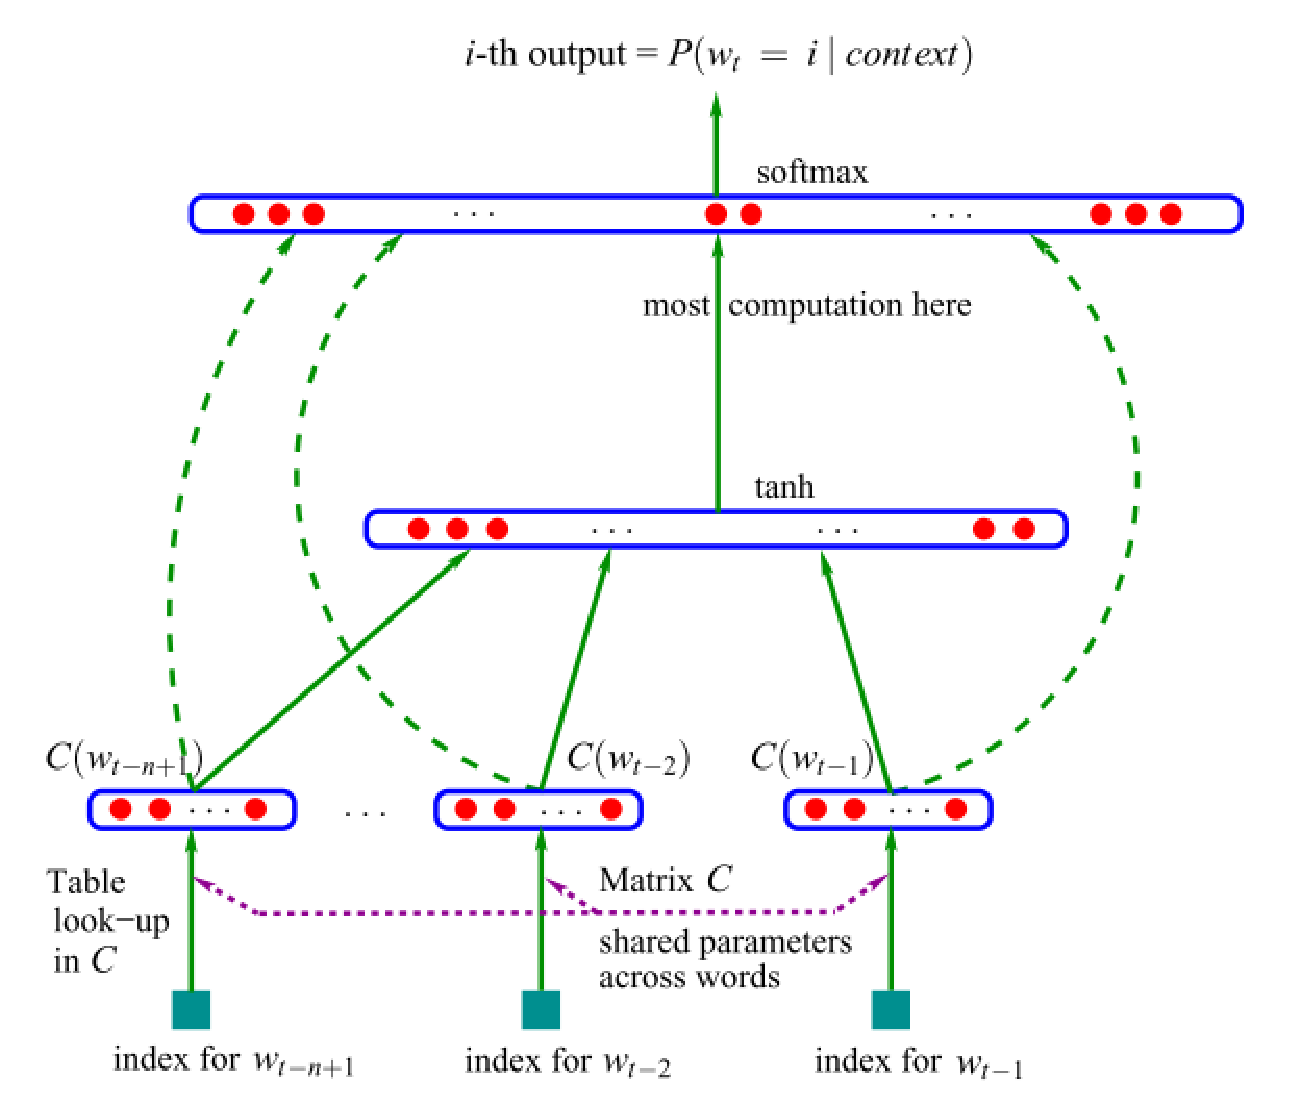
\includegraphics[width=.8\linewidth]{8_15_DL}\\
  \caption{An overview of the network architecture}\label{fig:DL}
\end{figure}

Figure \ref{fig:DL} shows the proposed neural architecture. The objective  function $f$ is a composition of $C$ and $g$, with $C$ being shared across all the words in the context. The function $g$ can be implemented by a feed-forward or recurrent neural network. This paper uses the ordinary hyperbolic tangent hidden layer with a softmax output layer.

The paper also explores parallelization on two types of platforms: shared-memory processor machines and Linux clusters with a fast network. In the case of a shared-memory processor, each processor works on a different subset of the data. Each processor computes the gradient for its examples, and performs stochastic gradient updates on the parameters of the model, which are simply stored in a shared-memory area. If the parallel computer is a network of CPUs, the paper chooses to parallelize across the parameters of the output units. The CPUs need to communicate the normalization factor of the output softmax, and the gradients on the hidden layer with the word feature layer. All the CPUs will duplicate the computations that precede the output units. After this step, each processor works on its local data as before.

In this experimental section, the paper measures the perplexity of the proposed model, and compares the results with several previous work. It is reported that the proposed method outperforms the most competitive alternative approach by up to 24\% in perplexity. 
\subsection{Stochastic language generation in dialogue using recurrent neural networks with convolutional sentence reranking \cite{Wen2015a}}

The task is to maps system acts into surface texts. The paper uses RNN LM to generate responses by sampling words from the predicted distribution conditioned on dialogue acts. After generating response candidates, CNN and RNN are used together to score and rerank the candidates. 
\subsection{Generating Text with Recurrent Neural Networks \cite{Martens2011}}

This paper proposes a new variant of \emph{Recurrent Neural Network (RNN)} called \emph{Multiplicative Recurrent Neural Network (MRNN)}, and demonstrates its power by applying it to character-level language modeling tasks. Specifically, the paper will use the MRNNs to predict the next character in a stream of text.

The standard RNN is formalized as follows: Given a sequence of input vectors $(x_1, ..., x_T)$, the RNN computes a sequence of hidden states $(h_1, ..., h_T)$ and a sequence of outputs $(o_1, ..., o_T)$ by iterating the following equations:
\begin{eqnarray}
h_t &=& tanh(W_{hx}x_t + W_{hh}h_{t-1} + b_h)\\
o_t &=& W_{oh}h_t + b_o
\end{eqnarray}

In the standard RNN the current input $x_t$ is first transformed via the weight matrix $W_{hx}$ and then contributes \emph{additively} to the hidden state, while the basic idea of MRNN is to allow the current input determine the entire hidden-to-hidden matrix ($W_{hh}$). Before going further, it is worthy to explain the motivation of this approach.

\begin{figure}[htbp]
  \centering
  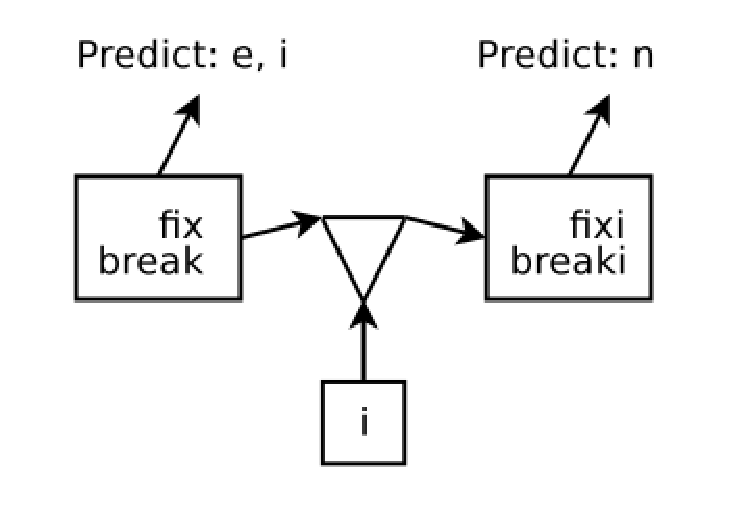
\includegraphics[width=.5\linewidth]{8_1_mrnn}\\
  \caption{A example that requires multiplicative connection}\label{fig:mrnn}
\end{figure}

For example in Figure \ref{fig:mrnn}, the character string ``ing'' is quite probable after ``fix'' and also quite probable after ``break''. If the hidden state vectors of the two words share a common concept of the stem of a verb, then there is a common representation to allow the character ``i'' to produce ``n''. Any evidence alone (verb stem or character ``i'') is not sufficient to make the prediction, and adding the weight additively is intuitively not a good strategy.

Based on the above analysis, in MRNN the update rule of hidden state vectors is changed to:
\begin{eqnarray}
h_t &=& tanh(W_{hx}x_t + W^{(x_t)}_{hh}h_{t-1} + b_h)
\end{eqnarray}
Here $W_{hh}$ is replaced with $W_{hh}^{(x_t)}$, allowing each character to specify a different hidden-to-hidden weight matrix.

The above scheme has a major drawback, which is that the storage required for $W_{hh}^{(x_t)}$ becomes prohibitive when the dimensionality of $x_t$ is even moderately large. The paper overcomes this problem by factoring $W_{hh}^{(x)}$ with three matrices $W_{fx}, W_{hf}$ and $W_{fh}$:
\begin{eqnarray}
W_{hh}^{(x_t)} = W_{hf} \cdot diag(W_{fx}x_t) \cdot W_{fh}
\end{eqnarray}
As a result, the updating rules can be represented as:
\begin{eqnarray}
f_t &=& diag(W_{fx}x_t) \cdot W_{fh}h_{t-1}\\
h_t &=& tanh(W_{hf}f_t + W_{hx}x_t)\\
o_t &=& W_{oh}h_t + b_o
\end{eqnarray}

In the experimental section, the paper makes comparison study with the \emph{sequence memorizer}  and \emph{PAQ}  methods. It is reported that MRNN achieves lower \emph{bits per character (bpc)} than the sequence memorizer but higher than PAQ (lower bpc implies better performance). The second part of experiment is to evaluate different methods with the \emph{debagging problem}, which is to convert a bag of words into a meaningful sentence. MRNN recovers the correct ordering 34\% of the time, which is higher than the memorizer (27\% of the time). Finally and most interestingly, the proposed neural network is used to generate sentence in character level, given a beginning of the sentence. For example, when initialized with the phrase ``The meaning of life is'', the MRNN generates the following sentence:

\begin{small}
The meaning of life is the tradition of the ancient human reproduction: it is less favorable to the good boy for when to remove her bigger. In the show's agreement unanimously resurfaced. The wild pasteured with consistent street forests were incorporated by the 15th century BE. In 1996 the primary rapford undergoes an effort that the reserve conditioning, written into Jewish cities, sleepers to incorporate the .St Eurasia that activates the population. Mar??a Nationale, Kelli, Zedlat-Dukastoe, Florendon, Ptuos thought is. To adapt in most parts of North America, the dynamic fairy Dan please believes, the free speech are much related to the...
\end{small}

\subsection{Recurrent Neural Network based Language Model \cite{Mikolov2010}}

This paper proposes a new \emph{recurrent neural network based language model (RNN LM)} with applications to speech recognition. Experimental results indicate that it reduces 50\% perplexity by using mixture of several RNN LMs, and speech recognition experiments show around 18\% reduction of word error rate on the Wall Street Journal task.

This paper uses an architecture that is usually called a \emph{simple recurrent neural network}, which is probably the simplest possible version of RNN, and very easy to implement and train. Let the input to the network at time $t$ be $x(t)$, output is denoted as $y(t)$, and $s(t)$ is the state of the network (hidden layer). Let $\oplus$ denote the concatenating operator. The simple recurrent neural network works by iterating the following equations:
\begin{align*}
x(t) &= w(t) \oplus s(t-1)\\
s_j(t) &= \sigma(\sum_i x_i(t) u_{ji})\\
y_k(t) &= softmax(\sum_j s_j(t) v_{kj})
\end{align*}

At each training step, error vector is computed according to cross entropy criterion and weighs are updated with the standard backpropagation algorithm.

The paper further suggests that the network should continue training even during testing phase, and refers to such model as \emph{dynamic}. While in training phase all data are presented to network several times in epochs, dynamic model gets updated just once as it processes testing data. It is shown that such simple technique is enough to obtain large perplexity reductions against static models. Dynamically updated models can thus automatically adapt to new domains.

In the experimental study, the paper evaluates the proposed method on several standard speech recognition tasks. On the WSJ corpus, the proposed model reduces WER by 18\% against 5-gram model with modified Kneser-Ney smoothing. Perplexity reductions are one of the largest ever reported (almost 50\%). In another experiment on the NIST RT05 corpus, it is shown that the proposed model trained on just 5.4M words can outperform backoff models that are trained on hundreds times more data.

\subsection{Energy-Based Models and Boltzmann Machines \cite{Bengio2009}}

In this survey we present the fifth chapter of the book \emph{Learning Deep Architectures for AI} by Bengio \cite{Bengio2009}. This chapter introduces the main mathematical concepts helpful to understand \emph{Restricted Boltzmann Machines (RBMs)}, which are particular energy-based models.

Energy-based models associate a scalar energy to each configuration of the variables of interest. For example, we would like plausible or desirable configurations to have low energy. The probability distribution of an energy-based model may be defined as follows:
\begin{equation}\label{equ:1}
P(x) = \frac{e^{-Energy(x)}}{Z}.
\end{equation}
Here $Z$ is a normalization term called the \emph{partition function} by analogy with physical systems.

In the \emph{products of experts} formulation, the energy function is a sum of terms, each one associated with an ``expert'' $f_i$:
\begin{equation}
Energy(x) = \sum_i f_i(x).
\end{equation}
Each expert can thus be seen as a detector of implausible configurations of $x$, or equivalently, as enforcing constraints on $x$.

In many cases we do not observe all the components simultaneously, or we want to introduce some non-observed variables to increase the expressive power of the model. So we consider an observed part $x$ and a hidden part $h$:
\begin{eqnarray}
P(x,h) = \frac{e^{-Energy(x,h)}}{Z},\\
P(x) = \sum_h P(x,h).
\end{eqnarray}
In order to map this formulation to the standard form, we introduce the notation of \emph{free energy}:
\begin{eqnarray}
P(x) = \frac{e^{-FreeEnergy(x)}}{Z},\\
FreeEnergy(x) = - \log \sum_h e^{-Energy(x,h)}.
\end{eqnarray}

The average log-likelihood gradient over the training set is
\begin{eqnarray}
E_{\hat{P}}[\frac{\partial \log P(x)}{\partial \theta}] = - E_{\hat{P}}[\frac{\partial FreeEnergy(x)}{\partial \theta}] + E_P[\frac{\partial FreeEnergy(x)}{\partial\theta}],
\end{eqnarray}
where expectations are over $x$, with $\hat{P}$ the training set empirical distribution and $E_P$ the expectation under the model's distribution.

If the energy can be written as a sum of terms associated with at most one hidden unit:
\begin{eqnarray}
Energy(x,h) = -\beta(x) + \sum_i \gamma_i(x, h_i),
\end{eqnarray}
then the free energy and numerator of the likelihood can be computed tractably:
\begin{eqnarray}
P(x) = \frac{e^\beta(x)}{Z} \prod_i \sum_{h_i} e^{-\gamma_i(x, h_i)}.
\end{eqnarray}

The \emph{Boltzmann machine} is a particular type of energy-based model with hidden variables. In a Boltzmann machine, the energy function is a general second-order polynomial:
\begin{eqnarray}
Energy(x,h) = -b'x - c'h - h'Wx - x'Ux - h'Vh.
\end{eqnarray}
The gradient of the log-likelihood can be written as:
\begin{eqnarray}
\frac{\partial \log P(x)}{\partial \theta} = - \sum_h P(h|x) \frac{\partial Energy(x,h)}{\partial \theta} + \sum_{\hat{x},h} P(\hat{x}, h) \frac{\partial Energy(\hat{x},h)}{\partial \theta}.
\end{eqnarray}
This gradient can be computed, if we have a procedure to sample from $P(h|x)$ and from $P(x,h)$. The basic idea is to use \emph{Gibbs sampling} in two phases: in the \emph{positive phase}, $x$ is clamped to the observed input vector, and we sample $h$ given $x$; in the \emph{negative phase} both $x$ and $h$ are sampled. Since two \emph{MCMCs (Monte Carlo Markov Chain)} (one for the positive phase and one for the negative phase) are needed for each example $x$, the computation can be very expensive.

\begin{figure}[h]
  \centering
  % Requires \usepackage{graphicx}
  \includegraphics[width=.6\linewidth]{Bengio09-RBM.png}\\
  \caption{Undirected graphical model of a RBM}\label{fig:Bengio09}
\end{figure}

In the \emph{Restricted Boltzmann Machine (RBM)}, the $h_i$ are independent of each other when conditioning on $x$, and the $x_j$ are independent of each other when conditioning on $h$ (cf. Figure \ref{fig:Bengio09}). The energy function is bilinear:
\begin{eqnarray}
Energy(x,h) = -b'x - c'h - h'Wx.
\end{eqnarray}
The free energy of the input can be computed efficiently:
\begin{eqnarray}
FreeEnergy(x,h) = -b'x - \sum_i \log \sum_{h_i} e^{h_i(ci + W_i x)}.
\end{eqnarray}
Using the same factorization trick, we can obtain a tractable expression for $P(h|x)$ and $P(x|h)$.

Gibbs sampling in fully connected Boltzmann Machines is slow because there are as many sub-steps in the Gibbs chain as there are units in the network. The Factorization enjoyed by RBMs bring two benefits: 1) we do not need to sample in the positive phase because the free energy is computed analytically; 2) the set of variables $(x,h)$ can be sampled in two sub-steps in each step of the Gibbs chain: first we sample $h$ given $x$, and then a new $x$ given $h$.

\emph{Contrastive Divergence (CD)} is an approximation of the log-likelihood gradient that has been found to be a successful update rule for training RBMs. The basic idea of $k$-step CD is simple, and involves a second approximation, which introduces some bias in the gradient: run the MCMC chain $x_1, ..., x_{k+1}$ for only $k$ steps starting from the observed example $x_1 = x$. The surprising empirical result is that even $k=1$ often gives good results.


\subsection{Three New Graphical Models for Statistical Language Modelling \cite{Mnih2007}}

This paper shows how real-valued distributed representations for words can be learned at the same time as learning a large set of stochastic binary hidden features that are used to predict the distributed representation of the next word from previous distributed representations. One of the proposed models significantly outperforms the best $n$-gram models.

The first model is called the \emph{Factored Restricted Boltzmann Machine Language Model (FRBM)}. Each word is represented using a real-valued feature vector of length $N_f$. Let $R$ be an $N_w \times N_f$ matrix with row $i$ being the feature vector for the $i$-th word. The \emph{joint energy} of a sequence of words $w_1, ..., w_n$ is defined as:
$$E(w_n, h; w_{1:n-1}) = -(\sum_{i=1}^n v_i^T R W_i)h.$$
Here matrix $W_i$ specifies the interaction between the vector of hidden variables and the feature vector.

The joint conditional distribution of the next word and the hidden configuration $h$ is defined in terms of the energy function as:
$$P(w_n, h | w_{1:n-1}) = \frac{1}{Z_c} \exp(-E(w_n,h; w_{1:n-1})),$$
where $Z_c$ is a context-dependent normalization term. The conditional distribution of the next word can be obtained by marginalizing over the hidden variables.
\begin{figure}
  \centering
  % Requires \usepackage{graphicx}
  \includegraphics[width=.6\linewidth]{Minh07-RBM.png}\\
  \caption{a) The diagram for FRBM and TFRMB. The dashed part is included only for the TFRBM; b) The diagram for the log-bilinear model.}\label{fig:Minh07-RBM}
\end{figure}

The second model is called the \emph{Temporal Factored RBM (TFRBM)}. The basic idea is to make a simple extension to the factored RBM language model. Suppose we want to predict word $w_{t+n}$ from $w_1, ..., w_{t+n-1}$ for some large $t$. The method applies a separate instance of the model to words $w_\tau, ..., w_{\tau+n-1}$ for each $\tau$ in $\{1, ..., t\}$. In order to propagate context information forward, it further introduces directed connections from $h^\tau$ to $h^{\tau+1}$, and computes the hidden state of model $\tau+1$ using the inputs from the hidden state of model $\tau$ as well as its visible units. Figure \ref{fig:Minh07-RBM} (a) shows the diagram for the temporal FRBM.

The third model is called the \emph{log-bilinear language model}. The energy function of this model is specified as:
$$E(w_n; w_{1:n-1}) = -(\sum_{i=1}^{n-1} v_i^T R C_i)R^T v_n - b_r^T R^T v_n - b^T_v v_n.$$
In the FRBM energy function the interaction is between the word feature vectors and the hidden variables, whereas in this model the interaction is between the feature vectors for the context words and the feature vector for the predicted word. Intuitively, the model predicts a feature vector for the next word by computing a linear function of the context word feature vectors. Then it assigns probabilities to all words in the vocabulary based on the similarity. This model is similar to the energy-based model proposed in \cite{Bengio2003A}. However, the model proposed here uses a bilinear energy function, while the energy function in \cite{Bengio2003A} is a one-hidden-layer neural network. Figure \ref{fig:Minh07-RBM} (b) shows a diagram of the log-bilinear language model.

In the experimental study, the paper evaluates the proposed models using the \emph{Associated Press News (APNews)} dataset consisting of a text stream of about 16 million words. In the first experiment, it is shown that three of the four network models are competitive with $n$-gram models. The best results were obtained by averaging with the temporal network model, resulting in 21\% reduction in perplexity over the best $n$-gram model. In the second experiment, it is also shown that the log-bilinear models clearly outperform the $n$-gram models.

